\documentclass[11pt]{article}

\usepackage[margin=0.92in]{geometry}
\usepackage[T1]{fontenc}
\usepackage{lmodern}
\usepackage{amsmath,amssymb}
\usepackage{array}
\usepackage{booktabs}
\usepackage{enumitem}
\usepackage{fancyhdr}
\usepackage{float}
\usepackage{hyperref}
\usepackage[protrusion=true,expansion=false]{microtype}
\usepackage{xcolor}
\usepackage{tikz}
\usetikzlibrary{arrows.meta,calc,decorations.pathreplacing,fit,matrix,positioning}

\hypersetup{
  colorlinks=true,
  linkcolor=blue!50!black,
  urlcolor=blue!50!black,
  citecolor=blue!50!black
}

\setlength{\parindent}{0pt}
\setlength{\parskip}{0.58em}
\setlist[itemize]{leftmargin=1.5em,itemsep=0.18em,topsep=0.25em}
\setlist[enumerate]{leftmargin=1.6em,itemsep=0.18em,topsep=0.25em}

\pagestyle{fancy}
\setlength{\headheight}{14pt}
\fancyhf{}
\lhead{\thepage}
\rhead{\itshape 15: LLM Serving and Inference}
\renewcommand{\headrulewidth}{0pt}
\cfoot{}

\definecolor{prefill}{RGB}{30,116,180}
\definecolor{decode}{RGB}{44,160,44}
\definecolor{cache}{RGB}{214,126,44}
\definecolor{queue}{RGB}{96,96,96}
\definecolor{lightblue}{RGB}{227,241,252}
\definecolor{lightgreen}{RGB}{228,246,226}
\definecolor{lightorange}{RGB}{255,239,221}
\definecolor{lightgray}{RGB}{242,242,242}

\newcommand{\kv}{\mathrm{KV}}
\newcommand{\HBM}{\mathrm{HBM}}
\newcommand{\SRAM}{\mathrm{SRAM}}
\newcommand{\EOS}{\texttt{<EOS>}}
\newcolumntype{L}[1]{>{\raggedright\arraybackslash}p{#1}}

\newcommand{\courseheader}{%
  \vspace*{0.35in}
  \begin{center}
  \fbox{%
    \begin{minipage}{0.94\textwidth}
    \vspace{0.6em}
    \textbf{CSE 291A/DSC 291: Data Systems for Machine Learning, Spring 2026}

    \vspace{1.2em}
    \begin{center}
    {\Large 15: LLM Serving and Inference: Batching, Speculation, and KV Cache Management}
    \end{center}
    \vspace{0.8em}
    \begin{tabular}{@{}p{0.12\textwidth}p{0.78\textwidth}@{}}
    \textit{Lecturer:} & \textit{Hao Zhang}\\
    \textit{Scribes:} &
    \textit{Suraj Ranganath, Vaishak Menon, Arunima Anand, Jackson Wilke, Atharv Nair, Rishika Mundada, Anish Patnaik, Kris Dcosta, Ishan Jain}
    \end{tabular}
    \vspace{0.6em}
    \end{minipage}%
  }
  \end{center}
  \vspace{1.2em}
}

\begin{document}
\thispagestyle{plain}
\courseheader

\section{Execution Model: Prefill, Decode, and the KV Cache}

The lecture started from the basic execution pattern of an autoregressive language model.  Given a prompt, the model first runs a \textbf{prefill} pass over all input tokens.  After that, it enters a \textbf{decode} loop.  Each decode iteration consumes the token generated in the previous iteration and produces exactly one new token.  The loop stops when the sequence reaches a maximum length or when the model emits a termination token such as \EOS.

This separation matters because prefill and decode stress the GPU in different ways.  In prefill, the sequence length can be large, so the model sees many tokens at once.  In decode, the effective sequence length for the current forward pass is one token.  The model is still large, but the batch of useful computation is small unless many requests are served together.

The key dimensions are batch size \(b\), sequence length \(s\), hidden size \(h\), number of heads \(n\), and per-head dimension \(d\).  Many tensors contain an \(s\) dimension.  Large \(s\) is expensive for attention because attention contains an \(s \times s\) interaction inside each sequence.  But \(s=1\) is also a problem when \(b\) is small: the GPU is asked to process one vector at a time.  The lecture emphasized this tension because it explains why the same model needs different optimization strategies under serving and single-request inference.

\begin{figure}[H]
\centering
\resizebox{\linewidth}{!}{%
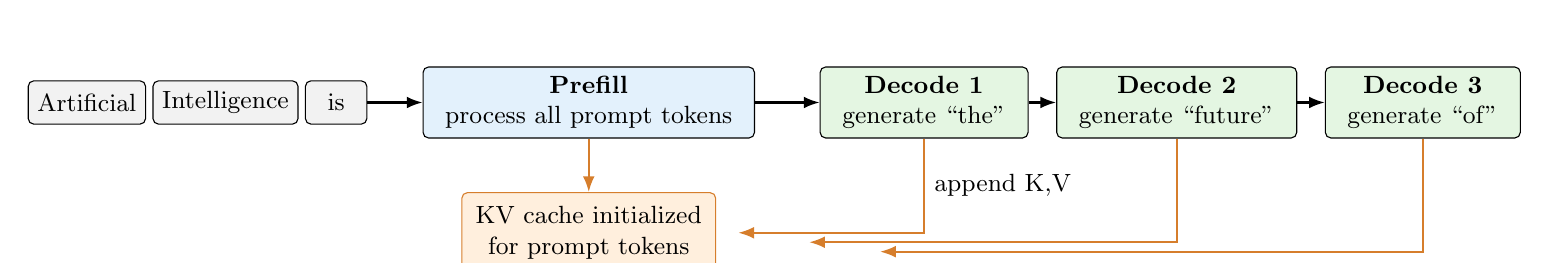
\begin{tikzpicture}[
  font=\small,
  box/.style={draw, rounded corners=2pt, minimum height=0.8cm, align=center, inner xsep=8pt},
  token/.style={draw, rounded corners=2pt, minimum height=0.55cm, minimum width=0.78cm, fill=lightgray},
  cachebox/.style={draw=cache, fill=lightorange, rounded corners=2pt, align=center, inner sep=5pt},
  arr/.style={-{Latex[length=2mm]}, thick}
]
\node[token] (a) at (0,0) {Artificial};
\node[token, right=0.08cm of a] (b) {Intelligence};
\node[token, right=0.08cm of b] (c) {is};
\node[box, fill=lightblue, right=0.7cm of c] (prefill) {\textbf{Prefill}\\process all prompt tokens};
\node[cachebox, below=0.68cm of prefill] (cache0) {KV cache initialized\\for prompt tokens};
\node[box, fill=lightgreen, right=0.82cm of prefill] (dec1) {\textbf{Decode 1}\\generate ``the''};
\node[box, fill=lightgreen, right=0.35cm of dec1] (dec2) {\textbf{Decode 2}\\generate ``future''};
\node[box, fill=lightgreen, right=0.35cm of dec2] (dec3) {\textbf{Decode 3}\\generate ``of''};
\draw[arr] (c) -- (prefill);
\draw[arr] (prefill) -- (dec1);
\draw[arr] (dec1) -- (dec2);
\draw[arr] (dec2) -- (dec3);
\draw[arr, cache] (prefill) -- (cache0);
\draw[arr, cache] (dec1.south) |- ($(cache0.east)+(0.28,0.0)$) node[pos=0.25, right, black] {append K,V};
\draw[arr, cache] (dec2.south) |- ($(cache0.east)+(1.18,-0.12)$);
\draw[arr, cache] (dec3.south) |- ($(cache0.east)+(2.08,-0.24)$);
\end{tikzpicture}
}
\caption{Autoregressive execution has one parallel prefill pass followed by a serial decode loop.  The KV cache stores per-layer keys and values so later decode steps do not recompute attention states for earlier tokens.}
\label{fig:prefill-decode}
\end{figure}

The \textbf{key-value cache} stores the attention keys and values produced by each transformer layer for every token that is still active.  During decode, a new query attends to all previous keys and values, then the new token's key and value are appended.  From a systems perspective this object is not a cache in the usual sense.  A cache normally trades on an uncertain hit rate.  The KV cache has a hit rate of essentially 100 percent: every future decode step needs the previous tokens.  It is better to think of it as the \textbf{working set} of active generation.

Its lifetime is also different from both parameters and ordinary activations.  Model weights are persistent for the whole server process.  Layer activations inside one forward pass are mostly ephemeral: a layer consumes them, produces the next activations, and the old values can be discarded.  KV entries sit between these extremes.  They are allocated at prefill, persist across all decode iterations for that request, grow by one token per decode step, and are freed only when the request finishes.

\section{Serving and Inference Are Different Regimes}

The lecture used \emph{serving} and \emph{inference} to distinguish two operating regimes.  The model computation is the same, but the performance objective is not.

\begin{center}
\begin{tabular}{@{}p{0.24\linewidth}p{0.34\linewidth}p{0.34\linewidth}@{}}
\toprule
Regime & Typical batch size & Main objective \\
\midrule
Online serving & Large effective batch size \(b\), because many users send requests to the same endpoint & High throughput and low cost per query, while meeting reasonable latency limits \\
Single-request inference & \(b=1\), or a very small batch & Low latency for a small number of requests \\
\bottomrule
\end{tabular}
\end{center}

In serving, the system is handling many independent requests.  Prompts arrive over time, have different lengths, and generate different numbers of output tokens.  The GPU should be kept busy across all of them.  In single-request inference, there may be no other user to batch with, so the main goal is to finish that one request as quickly as possible.

This is why large-\(b\) serving and \(b=1\) inference need different techniques.  Serving needs scheduling, dynamic batching, and memory management.  Single-request inference needs to reduce the number or cost of serial decode steps.

A practical way to remember the distinction is to ask what the expensive GPU is doing.  In hosted serving, the operator is paying for a fleet of GPUs and wants those GPUs to serve as many users as possible subject to latency constraints.  In local or edge inference, such as a laptop or phone running one assistant request, there may be no useful batch to form.  The bottleneck is not aggregate throughput; it is the latency of that one generation.

\section{Bottlenecks in Large-\texorpdfstring{\(b\)}{b} Serving}

For online serving, the first bottleneck is batching prompts of different lengths.  If request \(R_1\) has a 20-token prompt and request \(R_2\) has a 500-token prompt, the naive tensor shape is obtained by padding \(R_1\) to length 500.  That is simple, but it wastes compute on padding tokens.  In a high-throughput service, padding overhead directly lowers the number of useful tokens processed per second.

Decode has a different problem.  Each active request contributes only one new token per iteration, so the per-request sequence length for the current computation is \(s=1\).  However, the number of active requests \(b\) is large.  This large \(b\) prevents the main projections and MLPs from degenerating completely: the work is still closer to a matrix-matrix multiply (GEMM) than a matrix-vector multiply (GEMV), because the request dimension supplies useful parallelism.  The hard part is that the number of decode iterations is not known ahead of time.  One request may emit \EOS{} after a few tokens while another continues for hundreds of tokens.  A static batch has to wait for the longest request or leave GPU slots idle.

The memory bottleneck is the KV cache.  For each active request, the cache grows with the number of prompt and generated tokens.  With many concurrent users, total KV memory is approximately linear in the total number of active tokens.  If the cache is allocated or managed poorly, memory capacity becomes the limit before compute does.

The serving challenge can be summarized as:
\[
  \text{throughput} \quad \text{requires} \quad
  \begin{cases}
    \text{little or no padding in prefill},\\
    \text{dynamic replacement of finished requests},\\
    \text{KV cache storage proportional to useful active tokens}.
  \end{cases}
\]

\section{The \texorpdfstring{\(b=1\)}{b=1} Case and Speculative Decoding}

When \(b=1\), the prefill batching problem mostly disappears, but decode becomes a latency problem.  Each decode step processes one new token.  Large matrix multiplications become closer to matrix-vector operations, so the arithmetic intensity drops.  Informally,
\[
  \text{arithmetic intensity} = \frac{\text{operations}}{\text{bytes moved}}.
\]
With one token, the GPU cannot reuse model weights across many tokens or many requests.  The computation often becomes memory-bandwidth bound: each step repeatedly streams the model's weights from high-bandwidth memory into faster on-chip storage, performs a small amount of useful computation for one token, and then repeats.  This is why the lecture described the \(b=s=1\) case as wasteful even on very expensive accelerators such as B200-class GPUs.  The hardware has many SMs, but the current operation exposes too little parallel work to keep them busy.

The serial nature of autoregressive decoding gives a simple latency model:
\[
  \text{latency} = \text{step latency} \times \text{number of decode steps}.
\]
If one output token is generated per expensive target-model step, long generations are slow.  \textbf{Speculative decoding} attacks the second factor: it tries to generate and verify multiple tokens per target-model step.

The important constraint is algorithmic, not merely implementation-related.  Autoregressive generation cannot know token \(t+1\) until token \(t\) has been chosen.  A large model may therefore move hundreds of gigabytes of weights, or in trillion-parameter MoE settings a much larger active weight footprint, just to advance one token.  Speculative decoding does not remove autoregression; it changes how often the large target model has to perform this expensive step.

\subsection{How Speculative Decoding Helps}

The idea is to use a cheaper draft model to propose several future tokens, then use the large target model to verify them in one parallel pass.  For greedy decoding, the target model accepts the proposed tokens until the first position where the draft token differs from the target model's choice.  For sampling, the accept/reject rule is adjusted so the output distribution matches the target distribution.

\begin{figure}[H]
\centering
\resizebox{0.96\linewidth}{!}{%
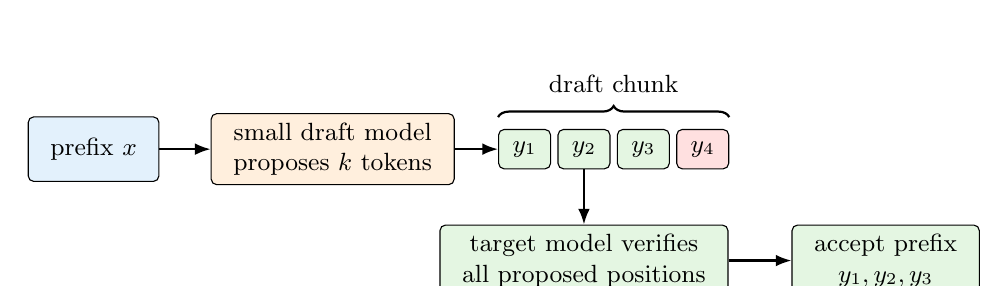
\begin{tikzpicture}[
  font=\small,
  stage/.style={draw, rounded corners=2pt, align=center, minimum height=0.82cm, inner xsep=8pt},
  tok/.style={draw, rounded corners=2pt, fill=lightgray, minimum width=0.66cm, minimum height=0.5cm},
  acc/.style={tok, fill=lightgreen},
  rej/.style={tok, fill=red!12},
  arr/.style={-{Latex[length=2mm]}, thick}
]
\node[stage, fill=lightblue] (prompt) {prefix \(x\)};
\node[stage, fill=lightorange, right=0.65cm of prompt] (draft) {small draft model\\proposes \(k\) tokens};
\node[acc, right=0.55cm of draft] (y1) {\(y_1\)};
\node[acc, right=0.08cm of y1] (y2) {\(y_2\)};
\node[acc, right=0.08cm of y2] (y3) {\(y_3\)};
\node[rej, right=0.08cm of y3] (y4) {\(y_4\)};
\node[stage, fill=lightgreen, below=0.7cm of y2] (verify) {target model verifies\\all proposed positions};
\node[stage, fill=lightgreen, right=0.8cm of verify] (accept) {accept prefix\\\(y_1,y_2,y_3\)};
\draw[arr] (prompt) -- (draft);
\draw[arr] (draft) -- (y1);
\draw[arr] (y2.south) -- (verify.north);
\draw[arr] (verify) -- (accept);
\draw[decorate, decoration={brace, amplitude=4pt}, thick]
  ($(y1.north west)+(0,0.15)$) -- ($(y4.north east)+(0,0.15)$)
  node[midway, above=5pt] {draft chunk};
\end{tikzpicture}
}
\caption{Speculative decoding trades extra draft-model work for fewer expensive target-model decode steps.  It is useful when target-model decode is memory-bandwidth bound and the draft acceptance rate is high.}
\label{fig:speculative}
\end{figure}

The target model still decides what is accepted.  The speedup comes from amortizing the target model's memory movement over several accepted tokens.  This is why speculative decoding is especially natural in the \(b=1\), \(s=1\) regime: the expensive model is underutilized per step, and reducing target steps can reduce end-to-end latency.

Speculation is not free.  It adds draft-model computation and can waste work if many proposed tokens are rejected.  Its benefit depends on three quantities: draft model speed, target model verification cost, and the average number of accepted tokens per verification pass.  The right mental model is that speculative decoding may increase total arithmetic, but it can reduce wall-clock latency because it amortizes the target model's memory movement over several accepted tokens.

\section{Static Batching Leaves Work on the Table}

The lecture then moved back to the large-\(b\) serving case.  Production systems improve GPU utilization by batching requests together, but a static batch is a poor fit for text generation.

The problem is easiest to see with the lecture's running example.  Suppose the serving engine can run at most three requests at once.  Requests \(R_1\) and \(R_2\) enter first.  Later, \(R_3\), \(R_4\), and \(R_5\) arrive.  If the system uses a static batch, it may keep running \(R_1\) and \(R_2\) until both finish.  If \(R_2\) emits \EOS{} early, its slot becomes idle.  If \(R_3\) arrives while the original batch is running, it may have to wait even though the GPU could have done useful work for it.

\begin{figure}[H]
\centering
\resizebox{0.92\linewidth}{!}{%
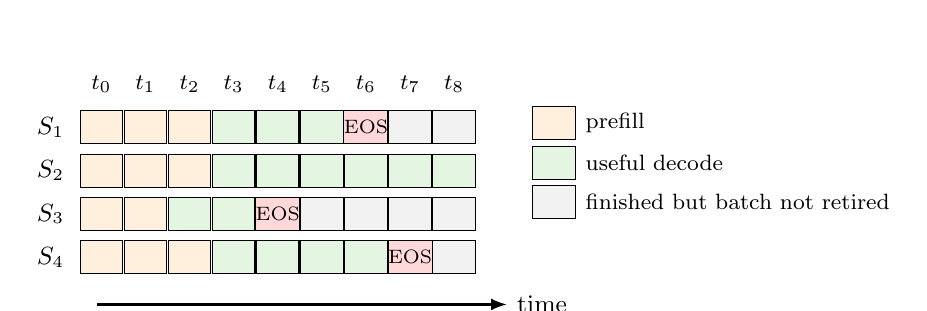
\begin{tikzpicture}[
  font=\small,
  cell/.style={draw, minimum width=0.54cm, minimum height=0.42cm, inner sep=0pt},
  pre/.style={cell, fill=lightorange},
  dec/.style={cell, fill=lightgreen},
  wait/.style={cell, fill=lightgray},
  eos/.style={cell, fill=red!15},
  axis/.style={-{Latex[length=2mm]}, thick}
]
\node[anchor=east] at (-0.35,0) {\(S_1\)};
\node[anchor=east] at (-0.35,-0.55) {\(S_2\)};
\node[anchor=east] at (-0.35,-1.10) {\(S_3\)};
\node[anchor=east] at (-0.35,-1.65) {\(S_4\)};
\foreach \x in {0,...,8} {
  \node[font=\footnotesize] at (\x*0.56,0.55) {\(t_{\x}\)};
}
\foreach \x in {0,1,2} \node[pre] at (\x*0.56,0) {};
\foreach \x in {3,4,5} \node[dec] at (\x*0.56,0) {};
\node[eos] at (6*0.56,0) {\scriptsize EOS};
\foreach \x in {7,8} \node[wait] at (\x*0.56,0) {};

\foreach \x in {0,1,2} \node[pre] at (\x*0.56,-0.55) {};
\foreach \x in {3,4,5,6,7,8} \node[dec] at (\x*0.56,-0.55) {};

\foreach \x in {0,1} \node[pre] at (\x*0.56,-1.10) {};
\foreach \x in {2,3} \node[dec] at (\x*0.56,-1.10) {};
\node[eos] at (4*0.56,-1.10) {\scriptsize EOS};
\foreach \x in {5,6,7,8} \node[wait] at (\x*0.56,-1.10) {};

\foreach \x in {0,1,2} \node[pre] at (\x*0.56,-1.65) {};
\foreach \x in {3,4,5,6} \node[dec] at (\x*0.56,-1.65) {};
\node[eos] at (7*0.56,-1.65) {\scriptsize EOS};
\node[wait] at (8*0.56,-1.65) {};
\draw[axis] (-0.05,-2.25) -- (5.15,-2.25) node[right] {time};
\node[pre, label=right:{\footnotesize prefill}] at (5.75,0.05) {};
\node[dec, label=right:{\footnotesize useful decode}] at (5.75,-0.45) {};
\node[wait, label=right:{\footnotesize finished but batch not retired}] at (5.75,-0.95) {};
\end{tikzpicture}
}
\caption{Static batching wastes iteration slots after shorter requests finish.  From the user's view, a request may have generated its answer but still wait for the longest request in the static batch.}
\label{fig:static-batching}
\end{figure}

Static batching therefore has three related issues:
\begin{itemize}
  \item requests complete at different decode iterations;
  \item finished requests leave idle GPU slots until the static batch drains;
  \item newly arrived requests cannot start immediately, increasing queueing latency.
\end{itemize}

\section{Continuous Batching}

\textbf{Continuous batching} fixes this by making the batch dynamic at each iteration.  A request pool on the CPU holds waiting work.  An execution engine on the GPU runs a batch of active work up to a configured capacity.  At every iteration, the scheduler can remove finished requests, admit newly arrived requests, and mix prefill and decode work.

The useful abstraction is \textbf{iteration-level scheduling}.  The batch is not a contract that lasts until every member finishes.  It is rebuilt at each iteration from the active requests and the waiting request pool.  This gives the system three abilities that static batching lacks: a finished request can leave immediately, a late request can join as soon as there is capacity, and a new prefill can run in the same iteration as ongoing decode work.

\begin{figure}[H]
\centering
\resizebox{\linewidth}{!}{%
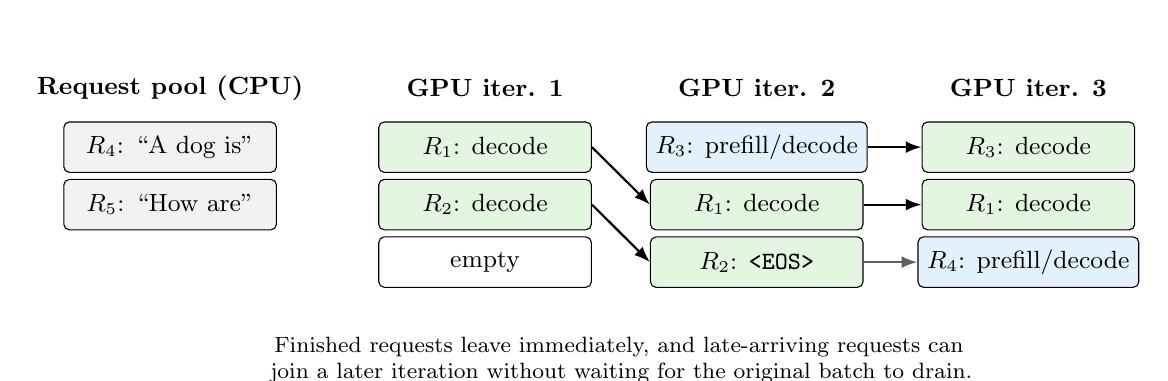
\begin{tikzpicture}[
  font=\small,
  slot/.style={draw, rounded corners=2pt, minimum width=2.7cm, minimum height=0.64cm, align=center},
  header/.style={font=\small\bfseries},
  arr/.style={-{Latex[length=2mm]}, thick}
]
\node[header] at (0,0.4) {Request pool (CPU)};
\node[slot, fill=lightgray] (q1) at (0,-0.35) {\(R_4\): ``A dog is''};
\node[slot, fill=lightgray] (q2) at (0,-1.08) {\(R_5\): ``How are''};

\node[header] at (4.0,0.4) {GPU iter. 1};
\node[slot, fill=lightgreen] (i1a) at (4.0,-0.35) {\(R_1\): decode};
\node[slot, fill=lightgreen] (i1b) at (4.0,-1.08) {\(R_2\): decode};
\node[slot, fill=white] (i1c) at (4.0,-1.81) {empty};

\node[header] at (7.45,0.4) {GPU iter. 2};
\node[slot, fill=lightblue] (i2a) at (7.45,-0.35) {\(R_3\): prefill/decode};
\node[slot, fill=lightgreen] (i2b) at (7.45,-1.08) {\(R_1\): decode};
\node[slot, fill=lightgreen] (i2c) at (7.45,-1.81) {\(R_2\): \EOS};

\node[header] at (10.9,0.4) {GPU iter. 3};
\node[slot, fill=lightgreen] (i3a) at (10.9,-0.35) {\(R_3\): decode};
\node[slot, fill=lightgreen] (i3b) at (10.9,-1.08) {\(R_1\): decode};
\node[slot, fill=lightblue] (i3c) at (10.9,-1.81) {\(R_4\): prefill/decode};

\draw[arr] (i1a.east) -- (i2b.west);
\draw[arr] (i1b.east) -- (i2c.west);
\draw[arr] (i2b.east) -- (i3b.west);
\draw[arr] (i2a.east) -- (i3a.west);
\draw[arr, queue] (i2c.east) -- (i3c.west);
\node[align=center, font=\footnotesize, text width=10.5cm] at (5.7,-3.05)
{Finished requests leave immediately, and late-arriving requests can join a later iteration without waiting for the original batch to drain.};
\end{tikzpicture}
}
\caption{Continuous batching follows the lecture's example: early exits and late arrivals are handled at iteration granularity.  The exact scheduler can be FIFO or more sophisticated, but the batch is not fixed for the lifetime of a request.}
\label{fig:continuous-batching}
\end{figure}

This design improves both utilization and user-facing latency.  The GPU sees a fuller batch over time, and each user can still receive an independent stream of tokens as soon as their request produces them.

The policy for choosing which requests enter the GPU is a scheduling problem.  A simple implementation may use FIFO, as in the lecture example where \(R_3\) enters before \(R_4\) and \(R_5\).  More advanced systems consider prompt length, remaining budget, priority, fairness, or latency service-level objectives.  The lecture's main point was not a particular policy, but the mechanism: the serving engine must be able to change the batch continuously.

One visible consequence is streaming.  Modern hosted LLM APIs often return tokens incrementally rather than waiting for the whole completion.  Continuous batching is one reason this is practical: each request can produce and return its own token stream while sharing GPU iterations with unrelated requests.

\section{How Ragged Requests Can Be Batched}

Continuous batching is only useful if the model computation can run efficiently on ragged requests.  The key observation from the lecture is that not every transformer operation depends on the sequence dimension in the same way.

Attention is sequence-dependent.  A token's attention output depends on which previous tokens it can attend to, and different requests may have different KV-cache lengths.  The attention kernel therefore needs per-request sequence metadata.

Many other transformer operations are token-dependent rather than sequence-dependent.  RMSNorm normalizes one token representation; the \(Q/K/V\) projections map one token hidden vector into attention vectors; the output projection, MLP, and SwiGLU/MoE feed-forward computation also apply per token.  For these operations, the system can collapse the ragged batch into a single list of tokens:
\[
  (b, s, h) \quad \longrightarrow \quad
  \left(\sum_i s_i, h\right).
\]
Then one large kernel processes all useful tokens, without padding shorter prompts to the longest prompt.

\begin{figure}[H]
\centering
\resizebox{0.92\linewidth}{!}{%
\begin{tikzpicture}[
  font=\small,
  tok/.style={draw, rounded corners=1pt, fill=lightgray, minimum width=0.45cm, minimum height=0.42cm},
  bluebox/.style={draw=prefill, fill=lightblue, rounded corners=2pt, align=center, inner sep=5pt},
  greenbox/.style={draw=decode, fill=lightgreen, rounded corners=2pt, align=center, inner sep=5pt},
  arr/.style={-{Latex[length=2mm]}, thick}
]
\node at (0,0.4) {\textbf{Ragged requests}};
\foreach \x in {0,1,2,3,4} \node[tok] at (\x*0.5,-0.2) {};
\node[left=0.08cm] at (-0.25,-0.2) {\(R_1\)};
\foreach \x in {0,1} \node[tok] at (\x*0.5,-0.78) {};
\node[left=0.08cm] at (-0.25,-0.78) {\(R_2\)};
\foreach \x in {0,1,2} \node[tok] at (\x*0.5,-1.36) {};
\node[left=0.08cm] at (-0.25,-1.36) {\(R_3\)};

\node[greenbox] (flat) at (4.25,-0.40) {token-wise kernels\\flatten \(\sum_i s_i\) tokens\\MLP/projections};
\node[bluebox] (attn) at (4.25,-1.72) {attention kernels\\sequence boundaries\\KV-cache metadata};
\draw[arr] (2.35,-0.78) -- (flat.west);
\draw[arr] (2.35,-0.98) -- (attn.west);

\node[draw, rounded corners=2pt, inner sep=4pt, right=0.85cm of flat] (tokens) {
  \begin{tikzpicture}[baseline=-0.5ex]
    \foreach \x in {0,...,9} \node[tok] at (\x*0.38,0) {};
  \end{tikzpicture}
};
\draw[arr] (flat) -- (tokens);
\node[align=center, font=\footnotesize, below=0.15cm of tokens] {one dense batch\\of real tokens};
\end{tikzpicture}
}
\caption{The system avoids padding by separating token-wise work from sequence-dependent attention.  This is why continuous batching can be effective when MLP/projection work dominates runtime.}
\label{fig:ragged}
\end{figure}

This decomposition also explains how different phases can be mixed:
\begin{itemize}
  \item \textbf{Prefill with prefill:} prompts have different lengths, so token-wise work can be flattened while attention uses ragged sequence boundaries.
  \item \textbf{Decode with decode:} each request contributes one query token, but those query tokens attend to KV caches of different lengths.
  \item \textbf{Prefill with decode:} new prompts and ongoing decode steps can share token-wise kernels, while attention handles full prompt attention for some requests and single-query attention for others.
\end{itemize}

The difficult implementation work is in the attention kernels and metadata management.  Modern serving engines such as vLLM and SGLang include kernels that support variable-length prefill, decode, and mixed prefill-decode batches.  The lecture emphasized the principle: do not force every operation into a padded rectangular tensor when the operation itself only needs a list of tokens.

This decomposition matters because, for large models at moderate context length, MLPs and projections often dominate the compute budget.  The lecture gave the rule of thumb that attention can be roughly 20--30\% of the work while MLP-like operations can be 70--80\%.  In that regime, batching token-wise work captures most of the benefit.  At very long context length the balance can flip, and attention can dominate.  That is why recent serving systems invest heavily in variable-length attention kernels rather than treating attention as an unbatched special case.

\subsection{Kernel Trend: Variable-Length Attention}

The current industry trend is to fuse more of this ragged attention logic into specialized GPU kernels.  Variable-length attention batching, online softmax as used in FlashAttention-style algorithms, and prefill/decode attention are increasingly handled together inside one kernel family.  This is less elegant than flattening token-wise MLP work because the kernel must track sequence boundaries, KV-cache locations, causal masks, and different context lengths.  But it is the direction production systems have moved because long contexts and mixed prefill-decode batches are now common.

The lecture highlighted FlashInfer as an example of this kernel-focused infrastructure layer.  Serving frameworks and training frameworks increasingly rely on libraries that provide optimized kernels for LLM inference, and sometimes diffusion workloads too.  The important takeaway is not a specific API, but the division of labor: high-level serving systems decide scheduling and memory layout, while specialized kernel libraries make ragged attention and token-level computation fast enough to keep expensive accelerators busy.

\begin{figure}[H]
\centering
\resizebox{0.96\linewidth}{!}{%
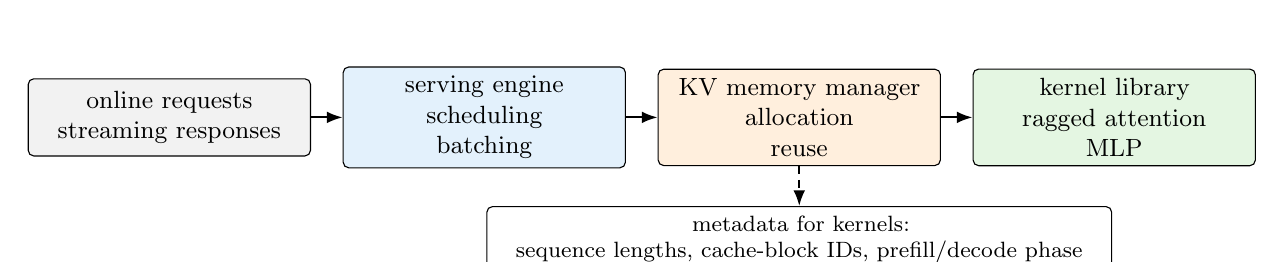
\begin{tikzpicture}[
  font=\small,
  layer/.style={draw, rounded corners=2pt, align=center, minimum height=0.98cm, text width=3.35cm},
  meta/.style={draw, rounded corners=2pt, align=center, font=\footnotesize, text width=7.7cm, fill=white},
  arr/.style={-{Latex[length=2mm]}, thick},
  metaarr/.style={-{Latex[length=2mm]}, thick, densely dashed}
]
\node[layer, fill=lightgray] (api) at (0,0) {online requests\\streaming responses};
\node[layer, fill=lightblue] (sched) at (4.0,0) {serving engine\\scheduling\\batching};
\node[layer, fill=lightorange] (mem) at (8.0,0) {KV memory manager\\allocation\\reuse};
\node[layer, fill=lightgreen] (kern) at (12.0,0) {kernel library\\ragged attention\\MLP};
\node[meta] (meta) at (8.0,-1.55) {metadata for kernels:\\sequence lengths, cache-block IDs, prefill/decode phase};
\draw[arr] (api) -- (sched);
\draw[arr] (sched) -- (mem);
\draw[arr] (mem) -- (kern);
\draw[metaarr] (mem.south) -- (meta.north);
\end{tikzpicture}
}
\caption{Modern serving stacks split responsibilities.  The scheduler decides which requests run; the memory manager decides where KV entries live; optimized kernel libraries execute token-wise and ragged attention work using the metadata supplied by the engine.}
\label{fig:serving-stack}
\end{figure}

\section{KV Cache Management}

For each transformer layer \(\ell\) and active request \(r\), the KV cache stores
\[
  K_{\ell}^{(r)}, V_{\ell}^{(r)}
  \in \mathbb{R}^{T_r \times n_{\kv} \times d_{\mathrm{head}}},
\]
where \(T_r\) is the number of cached tokens for that request, \(n_{\kv}\) is the number of key-value heads, and \(d_{\mathrm{head}}\) is the head dimension.  The factor of two is for keys and values.  For \(L\) layers and \(a\) bytes per element, the approximate memory use is
\[
  M_{\kv}
  \approx
  2 \cdot L \cdot n_{\kv} \cdot d_{\mathrm{head}} \cdot a
  \cdot
  \sum_{r \in \text{active}} T_r.
\]
Thus KV memory scales with the total number of active tokens, not only the number of active requests.  During decode, \(T_r\) grows by one per generated token.  When a request finishes, its KV memory should be released quickly.

\begin{figure}[H]
\centering
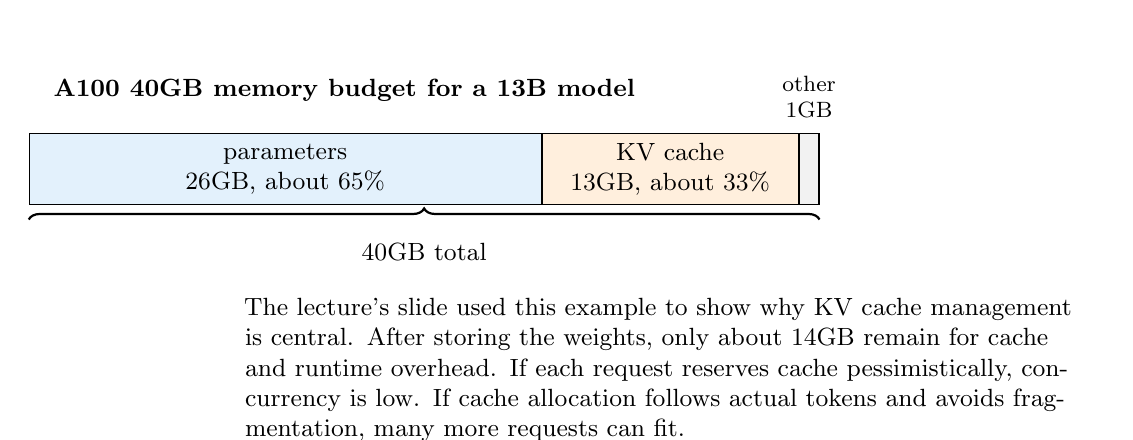
\begin{tikzpicture}[
  font=\small,
  mem/.style={draw, minimum height=0.9cm, align=center},
  label/.style={font=\small\bfseries}
]
\node[label] at (4.0,1.0) {A100 40GB memory budget for a 13B model};
\node[mem, fill=lightblue, minimum width=6.5cm] (param) at (3.25,0) {parameters\\26GB, about 65\%};
\node[mem, fill=lightorange, minimum width=3.25cm, right=0cm of param] (kv) {KV cache\\13GB, about 33\%};
\node[mem, fill=lightgray, minimum width=0.25cm, right=0cm of kv] (other) {};
\node[above=0.08cm of other, font=\footnotesize, align=center] {other\\1GB};
\draw[decorate, decoration={brace, amplitude=4pt}, thick]
  ($(param.south west)+(0,-0.18)$) -- ($(other.south east)+(0,-0.18)$)
  node[midway, below=5pt] {40GB total};
\node[align=left, text width=10.8cm, below=1.05cm of kv] {
The lecture's slide used this example to show why KV cache management is central.  After storing the weights, only about 14GB remain for cache and runtime overhead.  If each request reserves cache pessimistically, concurrency is low.  If cache allocation follows actual tokens and avoids fragmentation, many more requests can fit.
};
\end{tikzpicture}
\caption{In the 13B-on-A100 example, parameters dominate memory, but the remaining capacity is quickly consumed by KV cache.}
\label{fig:kv-memory}
\end{figure}

The A100 example is historically important because this was when KV-cache management became an obvious systems bottleneck.  Modern accelerators such as B200 provide much larger memory capacity, but the same structure remains: model weights claim a fixed base allocation, cache grows with active tokens, and throughput improves only if enough concurrent work fits in memory.

\begin{figure}[H]
\centering
\resizebox{0.92\linewidth}{!}{%
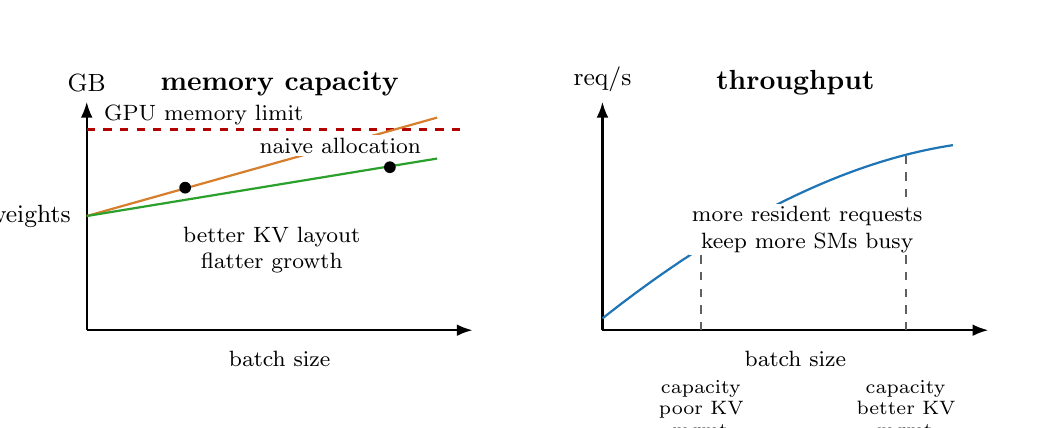
\begin{tikzpicture}[
  font=\small,
  axis/.style={-{Latex[length=2mm]}, thick},
  curve/.style={thick},
  dashedline/.style={dashed, thick},
  point/.style={circle, fill=black, inner sep=1.5pt}
]
\path[use as bounding box] (-0.75,-1.38) rectangle (11.85,3.35);
% Left plot: memory capacity
\node[font=\bfseries] at (2.45,3.13) {memory capacity};
\draw[axis] (0,0) -- (4.9,0);
\draw[axis] (0,0) -- (0,2.9) node[above] {GB};
\node[font=\footnotesize] at (2.45,-0.36) {batch size};
\draw[dashedline, red!70!black] (0,2.55) -- (4.75,2.55);
\node[font=\footnotesize, anchor=south west, fill=white, inner sep=1pt] at (0.18,2.56) {GPU memory limit};
\draw[curve, cache] (0,1.45) -- (4.45,2.70);
\draw[curve, decode] (0,1.45) -- (4.45,2.18);
\node[point] at (1.25,1.81) {};
\node[point] at (3.85,2.07) {};
\node[anchor=east] at (-0.08,1.45) {weights};
\node[align=center, font=\footnotesize, fill=white, inner sep=1pt] at (2.35,1.02) {better KV layout\\flatter growth};
\node[align=center, font=\footnotesize, fill=white, inner sep=1pt] at (3.22,2.34) {naive allocation};

% Right plot: throughput
\begin{scope}[xshift=6.55cm]
\node[font=\bfseries] at (2.45,3.15) {throughput};
\draw[axis] (0,0) -- (4.9,0);
\draw[axis] (0,0) -- (0,2.9) node[above] {req/s};
\node[font=\footnotesize] at (2.45,-0.36) {batch size};
\draw[curve, prefill] (0,0.15) .. controls (1.2,1.1) and (2.8,2.1) .. (4.45,2.35);
\draw[dashedline, queue] (1.25,0) -- (1.25,1.08);
\draw[dashedline, queue] (3.85,0) -- (3.85,2.25);
\node[font=\scriptsize, anchor=north] at (1.25,-0.52) {capacity};
\node[align=center, font=\scriptsize, text width=1.55cm, anchor=north] at (1.25,-0.78) {poor KV\\mgmt.};
\node[font=\scriptsize, anchor=north] at (3.85,-0.52) {capacity};
\node[align=center, font=\scriptsize, text width=1.55cm, anchor=north] at (3.85,-0.78) {better KV\\mgmt.};
\node[font=\footnotesize, align=center, fill=white, inner sep=1pt] at (2.60,1.28) {more resident requests\\keep more SMs busy};
\end{scope}
\end{tikzpicture}
}
\caption{KV-cache management links memory capacity to throughput.  If cache allocation grows too fast with batch size, the server hits the memory wall before the GPU reaches its useful throughput region.}
\label{fig:kv-throughput}
\end{figure}

A concrete calculation helps explain the slide's intuition.  For a 13B-class transformer with roughly \(L=40\), \(n_{\kv}=40\), \(d_{\mathrm{head}}=128\), fp16/bf16 cache elements, and a 2048-token sequence,
\[
  M_{\kv} \approx
  2 \cdot 40 \cdot 40 \cdot 128 \cdot 2 \cdot 2048
  \approx 1.6 \text{ GB per request}.
\]
Eight such full-length requests require about 13GB of KV cache, matching the memory scale shown in the lecture.  Better cache management can raise the number of concurrent requests by avoiding over-reservation and fragmentation.  The slides used the vLLM/PagedAttention story to preview the next lecture: existing systems in that example hit the wall around 8 concurrent requests, while vLLM-style cache management aims to support many more, on the order of 40 in the slide.  The systems lesson is not the exact number, which depends on model and workload, but the mechanism: flattening KV memory growth increases resident batch size, which raises throughput until another bottleneck appears.

A useful way to understand the PagedAttention preview is to separate the logical sequence from the physical KV-memory layout:
\begin{table}[H]
\centering
\small
\begin{tabular}{@{}L{0.24\linewidth}L{0.36\linewidth}L{0.34\linewidth}@{}}
\toprule
\textbf{Layout idea} & \textbf{What it means} & \textbf{Serving intuition}\\
\midrule
Contiguous reservation & Reserve KV space per request, often for an upper-bound output length. & Simple indexing, but unused tail space and fragmentation reduce the number of resident requests.\\
Block-based allocation & Store KV entries in fixed-size token blocks and use a block table to map logical token order to physical blocks. & The request behaves as if its cache is contiguous, while memory can grow only as real tokens arrive.\\
Throughput effect & Lower memory waste before the capacity wall. & Fits more resident requests, raising the effective batch size.\\
\bottomrule
\end{tabular}
\caption{PagedAttention borrows the virtual-memory idea of separating logical address order from physical storage.  For KV cache, this reduces fragmentation and over-reservation.}
\label{tab:paged-attention-intuition}
\end{table}

The lecture also mentioned prefix caching.  If many requests share a prefix, such as the same system prompt, their prefix KV states can be reused instead of recomputed and stored separately.  Serving engines often organize reusable prefixes with a trie or radix tree over token IDs.  This is separate from continuous batching, but it attacks the same serving objective: spend memory and compute only on useful, non-duplicated tokens.

\section{Takeaways}

The main conceptual split is between \textbf{latency optimization for small batches} and \textbf{throughput optimization for serving}.  In the \(b=1\) case, decode is serial and memory-bandwidth bound, so speculative decoding reduces the number of expensive target-model steps.  In large-\(b\) serving, the hard problems are dynamic batching and KV memory management.

Continuous batching improves serving by letting requests join and leave at iteration granularity.  Its implementation depends on separating token-wise transformer work from sequence-dependent attention.  The current kernel trend is to make even the sequence-dependent part less special, using variable-length attention kernels and FlashAttention-style online softmax inside production kernel libraries.  KV cache management is equally important because the cache grows with active tokens and can become the capacity bottleneck even when the GPU has enough compute.

The examples in lecture were meant to build this systems intuition.  Padding looks convenient, but wastes compute.  Static batches look simple, but waste slots and increase queueing.  KV cache management matters because it directly limits how many active users can fit on the GPU.  If many requests share the same prompt prefix, prefix caching and RadixAttention let the server reuse those KV entries instead of recomputing them or storing extra copies.

\end{document}
